
\documentclass[10pt,a4paper]{article}
%\usepackage[french]{babel}

\usepackage[dvips]{graphicx}
\usepackage{ifpdf}
\usepackage[dvips,
bookmarks,
bookmarksopen,
backref,
colorlinks,linkcolor={blue},citecolor={blue},urlcolor={blue},
]{hyperref}


\usepackage[T1]{fontenc}
\usepackage[latin1]{inputenc}
\makeatletter
\usepackage{graphicx}
\usepackage{color}
%\usepackage{pdfpages}
\oddsidemargin 0.25 in
\evensidemargin 0.25 in
\topmargin 0 in
\textwidth 6 in
\textheight 9 in
\parskip=4pt
\title{Functional description of the Neptune project EOS component graphical user interface}
\author{Marc Grandotto}
\date{\ }

\makeatother
\begin{document}

\pagestyle{empty}

\maketitle

\tableofcontents

\newpage
\section{Introduction}

This paper explains how the EOS GUI has been made and would like to be a guide to help further improvments.

As a matter of fact, the EOS GUI can be seen to be just an user of the EOS component. Its goal is to graphically (plot) show the thermodynamic properties variations of materials (fluids) as a function of one or two variables.

The GUI has been build in order to adapt itself automatically to the updates of the EOS component. Every things that are possible with the GUI belong from informations given by the EOS component (fluids, methods, thermodynamic quantities, etc.).

The GUI uses the only necessary EOS methods to its purpose.

The GUI calls the EOS C++ interface, but the GUI being written in Python (for fast and easy building tests convenience), a SWIG wrapping is used.

Naturally, this paper presents the C++ part then the Python part.

The graphical toolkit used is Qt4 (Salome standard). The plotting program used is ``gnuplot''. For two variables functions it is possible to write MED files (Salome standard). C++, Python and SWIG being also Salome standards, the EOS GUI is as close as possible to the Salome requirements.

\section{cpp directory}

\subsection{eosihmSrc1.hxx}

EosIhm class definition.

\subsection{eosihmSrc1.cxx}

EosIhm class implementation.

\begin{itemize}
\item putTheArrays : call eos2med.f, send the data to write a MED file.

\item getNumberOfValue : return the data ``nbval'', number of values.

\item initValueByStep : create an array with ``n+1'' values from ``a'' to ``b'' by step ``(b-a)/n''.

\item getValueAsList : no comment.

\item getErrorAsList : this is to get the field returned by the error manager.

\item getTheErrorI : return an error index.

\item getTheErrorC : return an error character string.

\item errorManaging : get the error parameters  from an  EOS\_Std\_Exception object and put them in the  EosIhm object .

\item computeValue : this is the main part ! We call the EOS component with the GUI data and we get the thermodynamic property value field. We use the ``compute'' method of the EOS object. Errors, if any, are catched.
\end{itemize}

\subsection{eosihm.i}

This is the SWIG interface.

It defines the  ``typemap'' (see the SWIG specialists). They are used to create an equivalence between types of different languages, here between Python and C++ (or C). Essentially we link integer or float arrays (int * or double *) with Python type ``list''.

It is close to the ``EosIhm'' class definition, so the reader will find more information in the C++ and Python parts. All the methods are interfaced but errorManaging.

\begin{itemize}
\item initValueByStep : called by eosRunFunction.py
\item getValueAsList : called by eosRunFunction.py
\item getErrorAsList : called by eosRunFunction.py
\item putTheArrays : called by eosRunFunction.py
\item getTheErrorI : called by eosRunFunction.py
\item getTheErrorC : called by eosRunFunction.py
\item computeValue : called by eosComponent.py
\item getNumberOfValue : called by eosComponent.py
\item createValue : unused (?)
\end{itemize}

\subsection{eos2med.f }

Write the MED file. 
\begin{itemize}
\item The mesh is a structured cartesian grid whose axes are the pressure and the enthalpy or the temperature. 
\item A field contains the computed thermodynamic property values.
\end{itemize} 

\subsection{eosihm.py}

This file is created by SWIG.

\section{Répertoire qt4}

\subsection{Python files}

Calling sequence :

\begin{tabular}{|l|l|l|l|}
\hline
eosMain4 & $\rightarrow$ eosGUI4 & $\rightarrow$ eosRunFunction & $\rightarrow$ eosComponent $\rightarrow$ \textsc{\textbf{le} composant \textcolor{red}{EOS}}\\
         &         &                & $\rightarrow$ eosPrint4     \\
 & & & \\
         &         & $\rightarrow$ eosAva         &  $\rightarrow$ eosUtil     \\
 & & & \\
         &         & $\rightarrow$ eosFileManager &             \\
         &         & $\rightarrow$ eosHelp4       &             \\
\hline
\end{tabular}

\subsubsection{eosMain4.py}

This is the entry point. It starts the interaction loop and creates an Ui\_NEPTUNE\_EOS object of the eosGUI4 module.

\subsubsection{eosGUI4a.py}

The name of the class is \textbf{Ui\_NEPTUNE\_EOS}.

The constructor starts the method \textbf{setupUi} which builds the graphical interface. This is the basic scheme proposed by the Qt4 interface generator (designer-qt4). This designer has been used to create a first design of the GUI. After that adjustments, updates and links to the methods are done manually. 

A widget ( window + gadget) is a visual element of a GUI (button, scrollbar, combo box, etc.).

\begin{itemize}
\item modiposi : change the origine (the upper left corner) of a widget.
\item resizeEvent : change the size of a widget.
\item retranslateUi : generated by the ``designer'', called by \textbf{setupUi}. Here are defined textes, colors, fonts, etc.
\end{itemize}

The following methods setup the link between a GUI action (``click'' or ``change'') and the corresponding running part of the interface.

\begin{itemize}
\item AddButton\_clicked
\item DeleteButton\_clicked
\item RedefButton\_clicked
\item HelpButton\_clicked
\item FileMButton\_clicked
\item GoButton\_clicked
\item QuitButton\_clicked
\item FunctionInformationButton\_clicked
\item Fluid\_changed
\item Method\_changed
\item Quantity\_changed
\end{itemize}


\subsubsection{eosRunFunction.py}

The name of the class is \textbf{EosRun}.

Quite all the work is done in the constructor.

It makes up the EOS component call, actually makes this call through ``eosComponent'', retrieves the results and plots (Plot option) (with gnuplot) or writes
 (Print option) (inside a popup window) the thermodynic property. The plot (or writing) associated file (.data file) is always written (Write to File option).

Several consistancy controls on the user inputs are done.

In order to use \textit{gnuplot}, a two (or three) columns file is written (.data file) together with a \textit{gnuplot} data file (.gpt file) that reads and plots the thermodynamic property values (.data  file).

2D plots are persistent, \textit{gnuplot} let back the handling to the user.

3D plots are not persistent, \textit{gnuplot} keeps the handling so 3D \textit{gnuplot} facilities are avalaible. The user has to manually close the \textit{gnuplot} window to get the handling on the GUI. 

(if someone knows a better solution, please let us know))

PostScript files are written by \textit{gnuplot} (\textit{gnuplot} can write other types of file but this is not the case here).

The \textbf{EosReadFile} class owns the ``External data'' thermodynamic method which is only a reading of the property values from a file. It is not yet implemented in the GUI.

\subsubsection{eosComponent.py}

The \textbf{EosComponent} class calls the EOS component to compute the thermodynamic properties defined by the user data.

The constructor gets the user data (detailOfFunction).
The ``compute'' method gets the values of the user data and calls the EOS component. This last appears as an object in the arguments. The called methods are \textit{computeValue, getNumberOfValue and getValueAsList}.

\subsubsection{eosAva.py}

The \textbf{EosAvailable} class gives the existing fluids, methods, references and thermodynamic properties available in the EOS component. It calls \textit{eosUtil} to build a dictionnary (Python type). This class is made to be asked. It owns the methods that build itself in reading the avalaible entities and the methods to answer to the requirement about what is possible or not.

\subsubsection{eosUtil.py}

The \textbf{eosUtil} class builds what is avalaible in the EOS component.

The  ``buildIndexDict'' method builds the availabilities dictionnary in reading an EOS file named ``index.eos''. This a two level dictionnary, first level keys are the fluid names, second level keys are the method names and the values are the reference names. So : D[fluid][method]=[ref list].

The ``buildPropDict'' method builds the available thermodynamic properties dictionnary in reading an EOS file named `` index.eos.properties''. The keys are the full property names and the values are the short property names (the one used inside the code).

\subsubsection{eosFileManager.py}

The EOS GUI writes several files. To, by default, keep the files the filenames end with a number which is automatically increased by one at each writing.
 
The \textbf{Ui\_FileManager} class is the manager of the written files (PostScript files .ps, thermodynamic property function data files .data, MED files .med). The class opens a window, creates lists of files through a filter using the suffixes and allows to remove one or several files. All the selection modes are possible (ExtendedSelection mode) using the keys Shift and Ctrl. 

\subsubsection{eosHelp4.py}

The \textbf{Ui\_Form2} class open a window and write inside it a text which is read on the file named eosHelp.txt. This is a resizeable window (resizeEvent method).

\subsubsection{eosPrint4.py}

Similar to eosHelp4, it would be possible to have only one module. 

Open a window and write inside it a text which can belong from an argument character string (\textbf{Ui\_Form4} class), or to be read on a file whose name is given as an argument (\textbf{Ui\_Form3} class).

\subsection{Pictures}

One can load only one picture (all-logos) or several pictures. The first case is used (see eosGUI4a.py).

\begin{itemize}
\item all-logos.png
\item l-areva.png
\item l-cea.png
\item l-edf.png
\item l-irsn.png
\item l-neptune.png
\item logo-neptune-site-hammi.png
\end{itemize}

\subsection{Texts}

This texts give short informations on the thermodynamic property computation methods. The text ``eosHelp'' is the on-line help.

\begin{itemize}
\item eosCathareInfo.txt
\item eosFlicaInfo.txt
\item eosHelp.txt
\item eosPerfectInfo.txt
\item eosRefpropInfo.txt
\item eosStiffenedInfo.txt
\item eosThetisInfo.txt
\end{itemize}

\section{Used Qt4 Classes}

(let see the Qt4 on-line documentation)

\begin{itemize}
\item QWidget
\item QMainWindow
\item QPixmap
\item QFrame
\item QLabel
\item QLineEdit
\item QPushButton
\item QRadioButton
\item QCheckBox
\item QListWidget : list of the defined functions, files list.
\item QAbstractItemView : abstract class owning list managing methods (select, move, etc.)
\item QComboBox : selecting fluids, methods, references, computed quantities, thermodynamic variables.
\item QGroupBox : gathering ``radio'' buttons (Derivative, Output type).
\item QTextBrowser : scrollable texts (scrollbar).
\item QApplication
\item QFont
\item QBrush
\item QColor
\item QPalette
\end{itemize}





\appendix

\section{Other files}

Ihm\_Diag.pdf :  Calling sequence in the EOS GUI.

%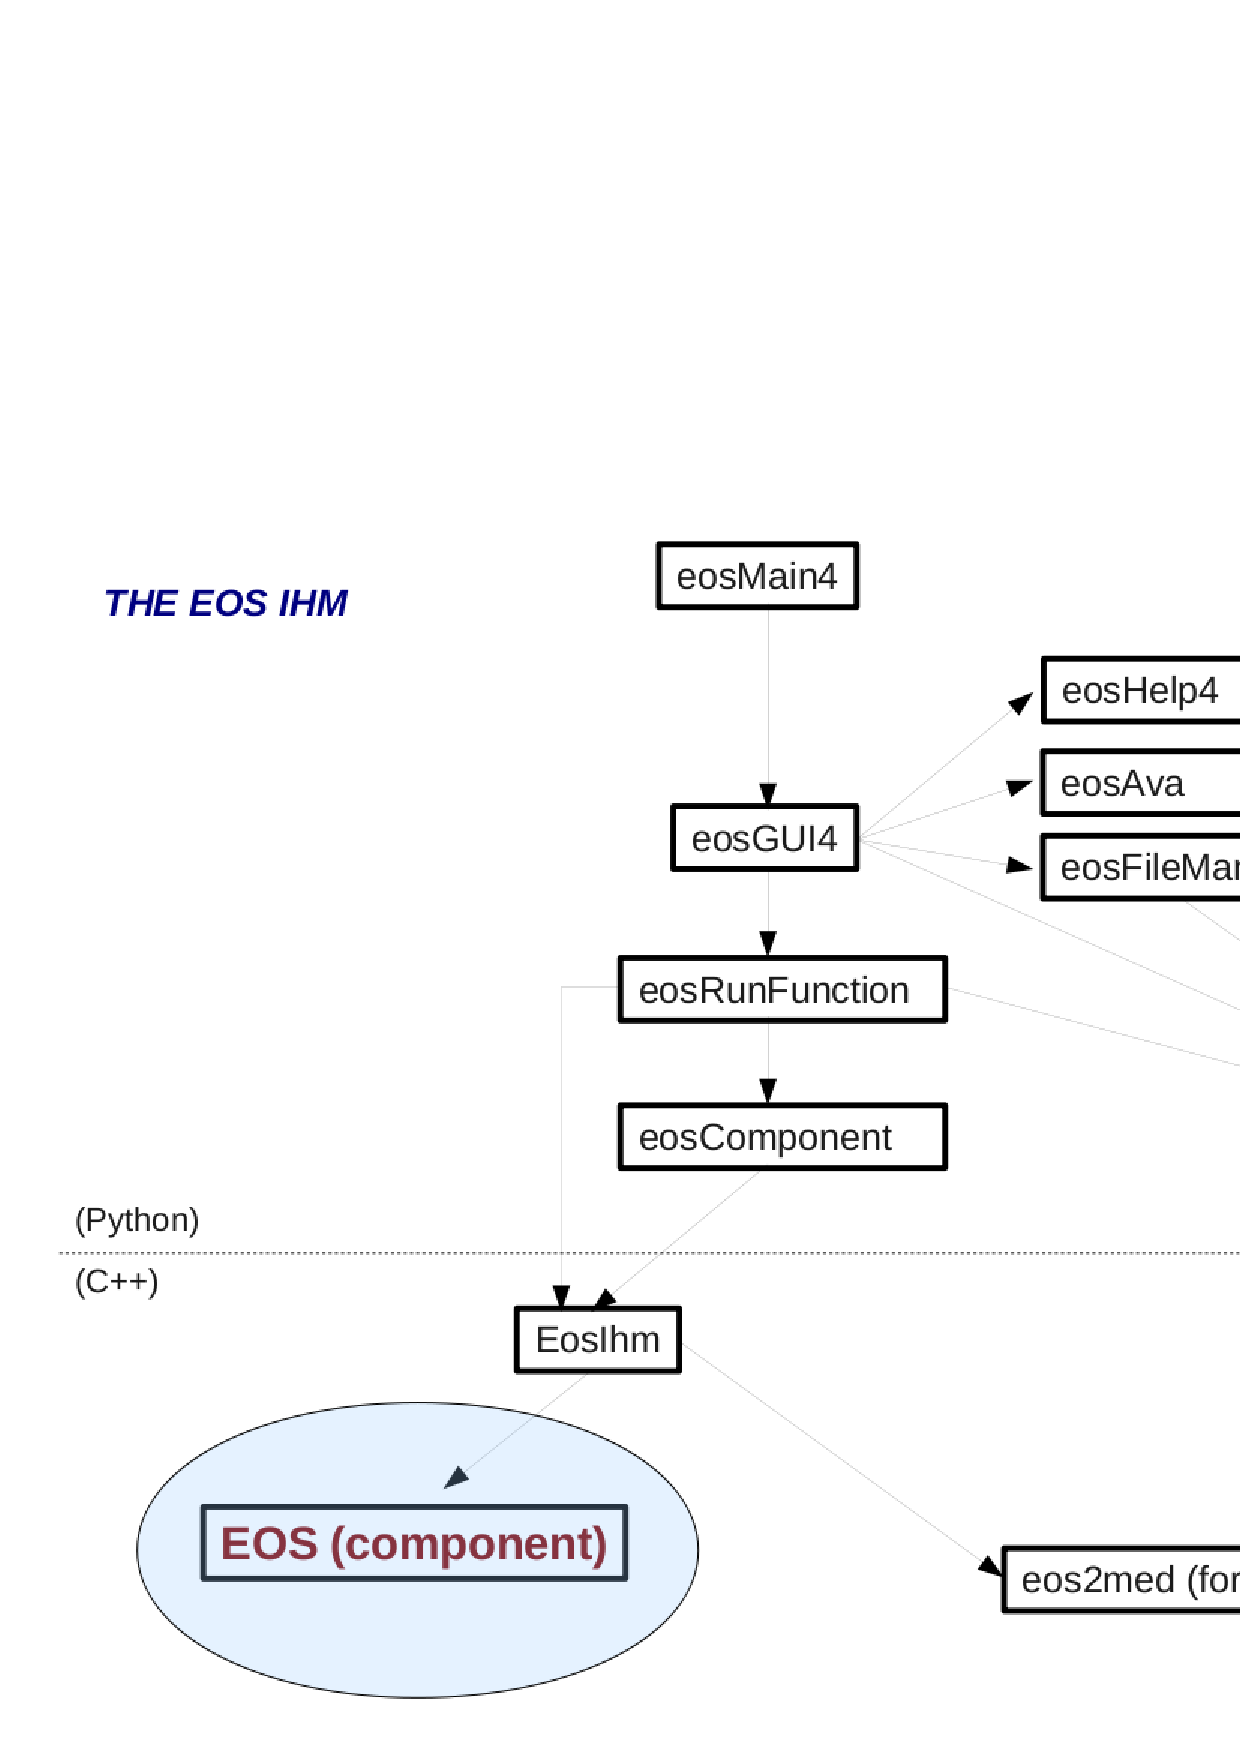
\includepdf{IhmDiag.pdf}
\begin{center}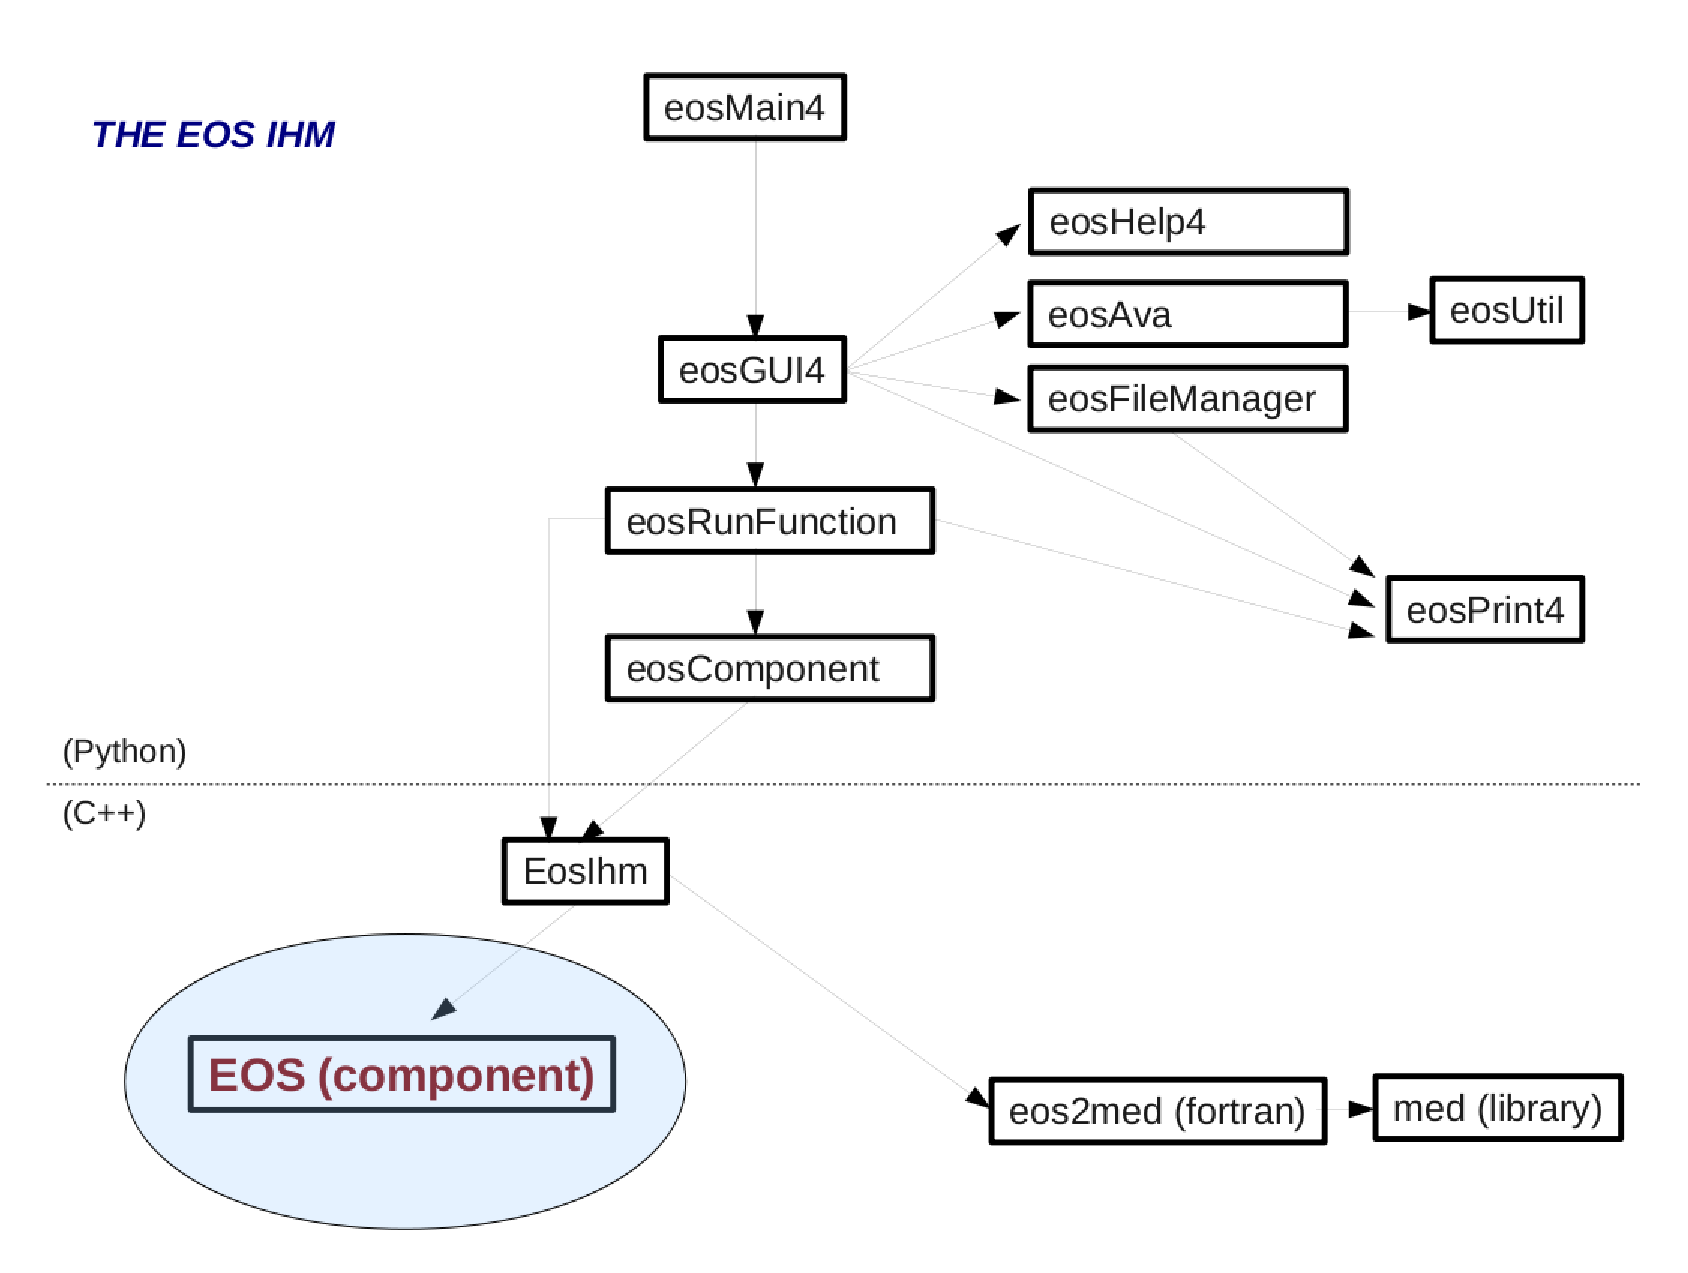
\includegraphics[width=10cm,angle=0]{IhmDiag.eps}\end{center}

\section{Exemple}

\begin{center}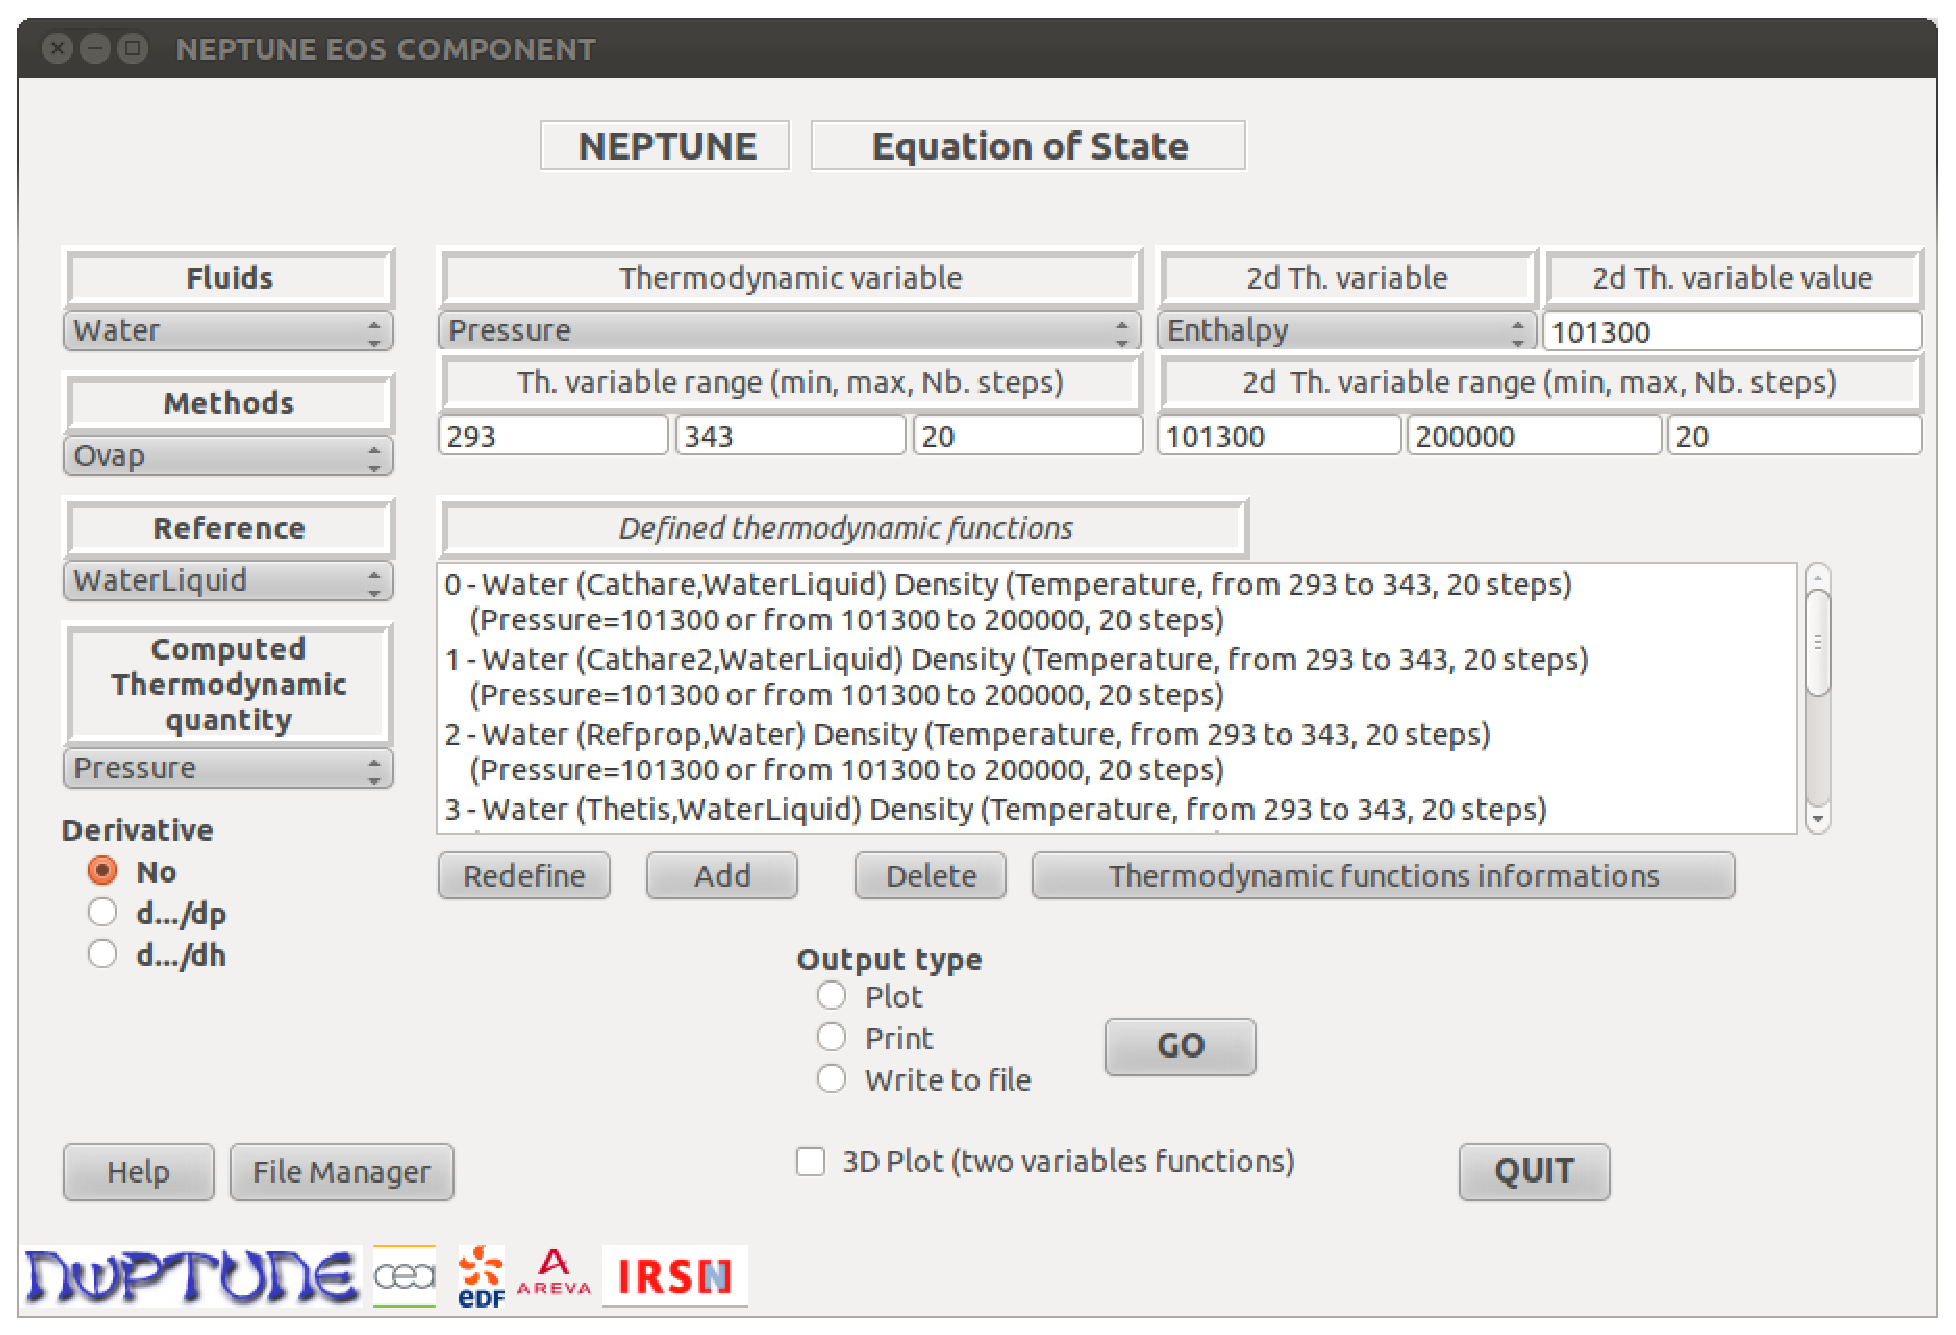
\includegraphics[width=20cm,angle=90]{CaptureEOS.eps}\end{center}

\end{document} 
